\chapter{Fourier Series and Transforms}
\vspace*{-1cm}
\begin{flushright}
\texttt{$2\pi$? Or not $2\pi$?}
\end{flushright}

The Fourier series and transform are among the most essential mathematical tools for physicists. \textcolor{red}{TO DO: Finish introduction...}

\textcolor{red}{Hereafter we assume that we are dealing with well behaved functions on their relevant domains. We shall restrict ourselves to the one-dimensinal cases. Generalizations are imediate.}

Every periodic function $f(x)$ can be expanded as a sum of trigonometric functions. If the period of the function is $\lambda$, i.e. $f(x+\lambda) = f(x)$, the \textbf{Fourier series} reads

\begin{equation}
 f(x) = \sum_{n=-\infty}^{\infty} c_n e^{-i k_n x},
 \label{eq:FourierSeries}
\end{equation}
where $k_n = 2\pi n/\lambda$, $n \in \mathbb{Z}$, and $e^{i\theta} = \cos\theta+i\sin\theta$. The coefficients $c_n$ are obtained from the orthogonality of the trigonometric functions, yielding

\begin{equation}
 c_n = \dfrac{1}{\lambda} \int_{x_0}^{x_0+\lambda} f(x) e^{i k_n x} dx.
 \label{eq:FourierSeriesInv}
\end{equation}
Here $x_0$ is arbitrary and the integral runs over one period of the function $f(x)$.

If the function $f(x)$ is not periodic, but we are interested in a finite domain $x \in [x_i,x_f]$, one can extend consider a periodic extension of $f(x)$ outside the domain, such that the Fourier series applies with the replacements $x_0 \rightarrow x_i$ and $\lambda \rightarrow x_f-x_i$. The periodic extension of $f(x)$ shall match the original function on the desired domain.

Consider now that the function $f(x)$ lives in the symmetric domain $x \in [-\frac{\lambda}{2}, \frac{\lambda}{2}]$, and we take the limit $\lambda \rightarrow \infty$. The discrete $k_n$ now become infinitesimally close, $\Delta k = k_{n+1}-k_n = \frac{2\pi}{\lambda} \rightarrow 0$, and become a continuous variable $k_n \rightarrow k$. Converting the sum in Eq.~\eqref{eq:FourierSeries} into an integral with $\sum_n \rightarrow \frac{\lambda}{2\pi}\int dk$, and replacing $c_n \rightarrow (\sqrt{2\pi}/\lambda)\tilde{f}(k)$, the Fourier series, Eq.~\eqref{eq:FourierSeries}, becomes

\begin{align}
 f(x) &= \dfrac{1}{\sqrt{2\pi}} \int_{-\infty}^{\infty} \tilde{f}(k) e^{-i k x} dk,\\
 \tilde{f}(k) &= \dfrac{1}{\sqrt{2\pi}} \int_{-\infty}^{\infty} f(x) e^{i k x} dx,
\end{align}
where $\tilde{f}(k) = F[f(x)]$ is the Fourier transform of $f(x)$, and reciprocally, $f(x) = F^{-1}[\tilde{f}(k)]$ is the inverse Fourier transform of $\tilde{f}(k)$.

The next example shows the Fourier series. Play with the function and parameters.

\begin{example}{Fourier Series}
\label{ex:FourierSeries}
\begin{minted}[escapeinside=||,mathescape]{julia}
using PyPlot

x = linspace(0.0, 30.0, 300); # domain
f(x) = sin(x)./x; # example function

lambda = x[end]-x[1]; # period
k(n) = 2pi*n/lambda; # wave number

# define a function to caculate the coefficients $c_n$
c(n) = quadgk(x->f(x)*exp(1im*k(n)*x), x[1], x[end])[1]/lambda;

N = 10; # the sum will be $\displaystyle \sum_{n=-N}^N$
Ni = -N:N; # array of values of $n$
Ci = [c(n) for n=Ni]; # calculate the coefficients and store in an array

# combine the arrays to recover the approximate function
fa=sum(i-> Ci[i]*exp(-1im*k(Ni[i])*x), 1:(2*N+1))

clf(); # the plot is shown in $\text{Fig. \ref{fig:FourierSeries}}$
subplot2grid((2,2),(0,0),colspan=2)
plot(x,f(x)); # plot the original function
plot(x, real(fa)) # and the approximated one
xlabel(L"$ x $");
ylabel(L"$ f(x) $");

subplot2grid((2,2),(1,0))
vlines(Ni, 0, real(Ci)); # real part of $c_n$
scatter(Ni, real(Ci));
xlabel(L"$ n $")
ylabel(L"$ Re\{c_n\} $")

subplot2grid((2,2),(1,1))
vlines(Ni, 0, imag(Ci)); # imaginary part of $c_n$
scatter(Ni, imag(Ci));
xlabel(L"$ n $")
ylabel(L"$ Im\{c_n\} $")

tight_layout();
\end{minted}
\end{example}

\begin{figure}[ht!]
 \centering
 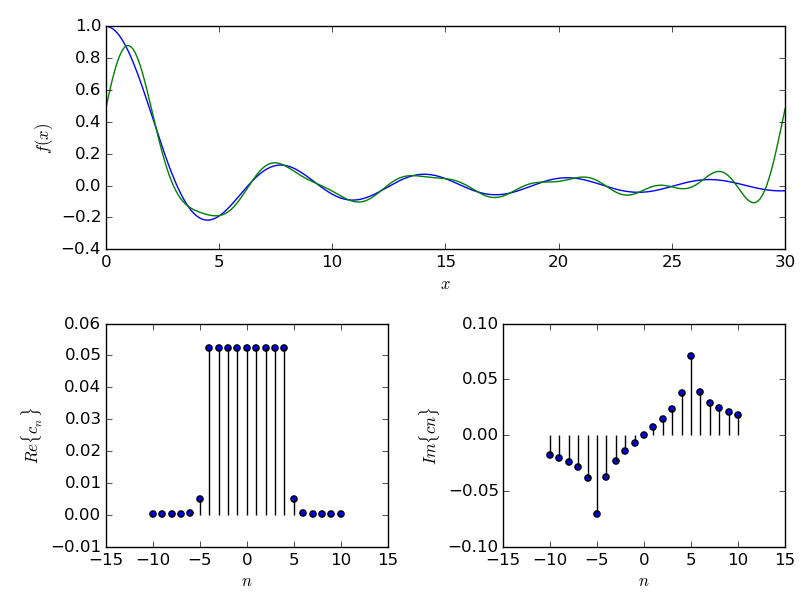
\includegraphics[width=14cm,keepaspectratio=true]{./FourierSeries.png}
 \caption{Output of Example \ref{ex:FourierSeries}.}
 \label{fig:FourierSeries}
\end{figure}

Typically, when we work with a function $f(x)$, where $x$ is a space coordinate, the Fourier transform is set in terms of the wave-number $k$ as above. If our signal is a function of time, i.e. $f(t)$, the Fourier transform is usually set in terms of the angular frequency $\omega$ as $\tilde{f}(\omega) = F[f(t)]$. 

\section{General properties of the Fourier transform}

There are many important properties of the Fourier transform that can be applied to solve physics problems. Here I'll list (without demonstrations) a few properties that will be useful for us in this Chapter. 

\subsubsection*{Linearity}

Let $f(x) = A g(x) + B h(x)$, the Fourier transform of $f(x)$ is $\tilde{f}(k) = A \tilde{g}(k) + B \tilde{h}(k)$.

\subsubsection*{Translation}

For a constant shift $x_0$ in $f(x) = g(x-x_0)$, we get $\tilde{f}(k) = e^{-i x_0 k}\tilde{g}(k)$.
Equivalently, a phase set by $k_0$ as $f(x) = e^{i k_0 x} g(x)$ leads to a Fourier transform shifted in the reciprocal space $\tilde{f}(k) = g(k-k_0)$.

\subsubsection*{Scaling}

For a real number $A$ in $f(x) = g(Ax)$, the Fourier transform scales as $\tilde{f}(k) = \frac{1}{|A|}\tilde{g}(k/A)$.

\subsubsection*{Derivatives}

Let $f_n(x) = \frac{d^n}{dx^n}g(x)$ denote the $n$-th derivative of $g(x)$, the transform is $\tilde{f}_n(k) = (ik)^n\tilde{g}(k)$.

\noindent
Equivalently, for $f(x) = x^n g(x)$, the transform is $\tilde{f}(k) = i^n \frac{d^n}{dk^n}\tilde{g}(k)$.

\subsubsection*{Convolution}

The convolution of the functions $g(x)$ and $h(x)$ is

\begin{equation}
 f(x) = (g\ast h)(x) = \int_{-\infty}^{\infty}g(x')h(x-x')dx'.
\end{equation}

The Fourier transform of a convolution is $\tilde{f}(k) = \sqrt{2\pi}\tilde{g}(k)\tilde{h}(k)$, which is simply the product of Fourier transformed functions. Conversely, if the function is the product of $g(x)$ and $h(x)$, i.e. $f(x) = g(x)h(x)$, the Fourier transform is $\tilde{f}(k) = (\tilde{g}\ast\tilde{h})/\sqrt{2\pi}$.


\section{Numerical implementations}

\subsection{Discrete Fourier Transform (DFT)}

The Discrete Fourier Transform is equivalent to the Fourier series applied on a discrete $x$ lattice. It can be obtained from Eqs.~\eqref{eq:FourierSeries}-\eqref{eq:FourierSeriesInv} for $x_0 = 0$, $dx = \lambda/N$, $x \rightarrow x_n = n\lambda/N$, and converting the integral in Eq.~\eqref{eq:FourierSeriesInv} into a sum.

Let $f$ be an array with $N$ elements representing the function $f(x)$. The Fourier transform $\tilde{f}(k) = F[f(x)]$ is represented by an array $\tilde{f}$ whose elements are

\begin{equation}
 \tilde{f}_m = \sum_{n=1}^N f_n \exp\left[-i \dfrac{2\pi(n-1)(m-1)}{N}\right].
\end{equation}

Conversely, given a vector $\tilde{f}$ representing a function $\tilde{f}(k)$ in k-space, the inverse Fourier transform $f(x) = F[\tilde{f}(k)]$ is represented by the array $f$ with elements

\begin{equation}
  f_n = \dfrac{1}{N} \sum_{m=1}^N \tilde{f}_m \exp\left[+i \dfrac{2\pi(m-1)(n-1)}{N}\right].
\end{equation}

Since we have to calculate all elements to compose the full array $\tilde{f}$ or $f$, the DFT or the inverse DFT takes $N^2$ operations. In contrast, the \texttt{Fast Fourier Transform} (FFT) algorithm takes $N\log_2 N$ operations, which is much smaller than $N^2$ for large $N$.

\subsection{Fast Fourier Transform (FFT)}

\red{(TO DO)} Here I'll follow the Radix-2 code of Cooley-Tukey: \url{https://en.wikipedia.org/wiki/Cooley%E2%80%93Tukey_FFT_algorithm}


\subsection{Julia's native FFT}

Julia comes with a native implementation of FFT via the efficient FFTW library\footnote{FFTW: \url{http://www.fftw.org/}}. We have implicitly used the FFT before when using the command \texttt{conv} to perform convolutions. The main commands to remember are \texttt{fft}, \texttt{ifft}, \texttt{fftshift}, and \texttt{ifftshift}.

These functions act on arrays. Therefore, hereafter consider a discrete domain (\texttt{linspace)} $x$ with spacing $\Delta x$ and the array $f(x) \rightarrow f$ set on this domain. 

\begin{figure}[ht!]
 \centering
 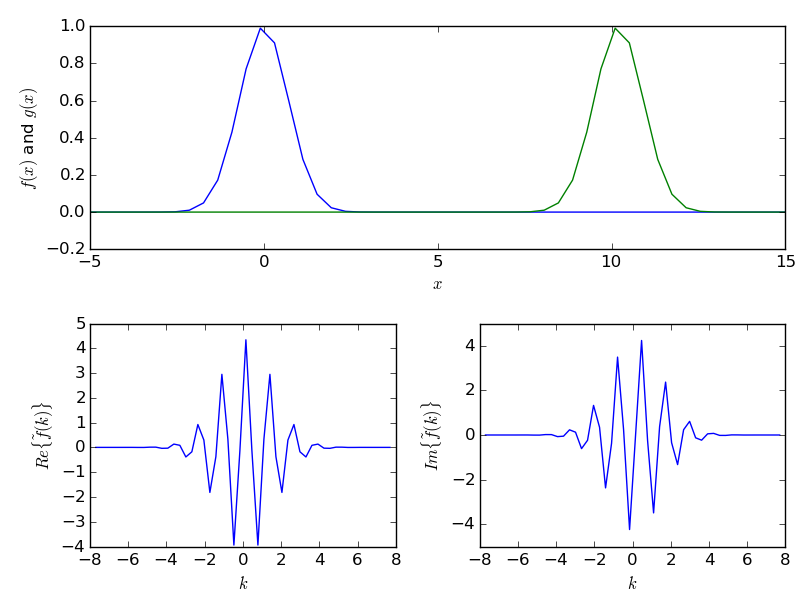
\includegraphics[width=14cm,keepaspectratio=true]{./FTShift.png}
 \caption{Output of Example \ref{ex:FTShift}.}
 \label{fig:FTShift}
\end{figure}

First, the command \texttt{fft} acts on an array $f$ and returns its Fourier transform $\tilde{f}$. Reciprocally, the command \texttt{ifft} acts on the array $\tilde{f}$ and returns its inverse Fourier transform $f$.

Notice that the array $f$ represents the function $f(x)$ over the discrete domain set by the array $x$. Conversely, the array $\tilde{f}$ represents the Fourier transformed function $\tilde{f}(k)$. The FFT implementation defines the domain of reciprocal space as $k \in [0, \frac{2\pi}{\Delta x})$. However, due to the periodicity of the Fourier transforms, the region $\frac{\pi}{\Delta x} \leq k < \frac{2\pi}{\Delta x}$ is actually equivalent to the region $-\frac{\pi}{\Delta x} \leq k < 0$. Typically, it is more interesting to work on the reciprocal space in the symmetric domain $k \in [-\frac{\pi}{\Delta x}, \frac{\pi}{\Delta x})$. 

One can use the commands \texttt{fftshift} and \texttt{ifftshift} to switch between these choices of domains above. The \texttt{fftshit} converts the domain from $k \in [0, \frac{2\pi}{\Delta x})$ into $k \in [-\frac{\pi}{\Delta x}, \frac{\pi}{\Delta x})$, while \texttt{ifftshift} performs the inverse operation.

The next example uses the translation property of the Fourier transform to shift a function by $x_0$. Check also Problem \ref{prob:FFTdiff}.

\begin{example}{Fourier transform using the FFT}
\label{ex:FTShift}
\begin{minted}[escapeinside=||,mathescape]{julia}
using PyPlot

n = 50; # using a small number of points for better visualization
x = linspace(-5.0, 15.0, n); # $x$ domain
dx = x[2]-x[1]; # spacing $\Delta x$
k = linspace(-pi/dx, pi/dx, n); # $k$ domain (symmetric)

# function in x-space
f = exp(-x.^2); # example function

# function in k-space
# and using fftshift to put ft in the symmetric domain
ft = fftshift(fft(f)); 

x0 = 10; # let's shift the function
gk = ft.* exp(-1im*x0*k); # see the Fourier transform properties
# goes back to the $[0,\frac{2pi}{dx})$ k-domain and apply ifft
g = ifft(ifftshift(gk)); 
# $g(x) = F^{-1}\big[ e^{-ix_0k}\tilde{f}(k)\big]$

clf(); # the plot is shown in $\text{Fig. \ref{fig:FTShift}}$
subplot2grid((2,2),(0,0),colspan=2)
plot(x,f); # plot the original function
plot(x, real(g)) # and shifted one
xlabel(L"$x$");
ylabel(L"$f(x)$ and $g(x)$")

# plot the real part of the Fourier transform
# shifting to the symmetric $k$-domain
subplot2grid((2,2),(1,0))
plot(k, real(ft));
xlabel(L"$k$")
ylabel(L"$Re\{\tilde{f}(k)\} $")

# plot the imaginary part of the Fourier transform
# shifting to the symmetric $k$-domain
subplot2grid((2,2),(1,1))
plot(k, imag(ft));
xlabel(L"$k$")
ylabel(L"$Im\{\tilde{f}(k)\} $")

tight_layout();
\end{minted}
\end{example}

\section{Applications of the FFT}

\subsection{Spectral analysis and frequency filters}

Let $\tilde{f}(\omega) = F[f(t)]$ be the Fourier transform of $f(t)$. The power spectrum of $f(t)$ is $S(\omega) = |\tilde{f}(\omega)|^2$. The plot of $S(\omega)$ \textit{vs} $\omega$ shows us which components (frequencies $\omega$) of the Fourier transform contribute to the signal $f(t)$. The power spectrum characterizes the color of a light beam, and the timbre of a musical instrument.

If our signal is simply $f(t) = A \sin(\omega_0 t)$, its Fourier transform is 

\begin{equation}
\tilde{f}(\omega) = i A \sqrt{\dfrac{\pi}{2}}\Big[\delta(\omega-\omega_0)-\delta(\omega+\omega_0)\Big],
\end{equation}
and the power spectrum will show two $\delta$-peaks at $\omega = \pm \omega_0$. This is the expected solution of the simple pendulum in the harmonic regime. Check Problem \ref{prob:FFTpendulum}.

\subsubsection{Noise and frequency filters}

What if our signal was noisy? There are many types of noise depending on their source\footnote{\href{https://en.wikipedia.org/wiki/Colors\_of\_noise}{The colors of noise (Wikipedia)}}. Musical instruments may suffer from high frequency noises due to electronic systems, bad cables, etc. The type of noise is defined by its power spectrum. For instance, a \textit{white noise} shows a constant power spectrum will all frequencies contributing equally. Hence the name \textit{white noise} as a reference to white light. The power spectrum of a \textit{pink noise} decays with $1/\omega$ and appears in most natural phenomena. The types of noise got their names as colors due to the initial analogy of white noise and white light.

In the next example, let's artificially generate and eliminate a white noise. The result is shown if Fig.~\ref{fig:whitenoise}. The white noise in this example have a power spectrum $S(\omega) \approx 10$, and two signal peaks show at $\omega = \pm 2\pi$. To filter the white noise we simply collect only the fft components that are above the white noise power spectrum.

\begin{example}{White noise}
\label{ex:whitenoise}
\begin{minted}[escapeinside=||,mathescape]{julia}
using PyPlot

N=300000; # generate signal with large number of points
t=linspace(0, 30, N); # time domain
dt=t[2]-t[1];
w=linspace(0, 2pi/dt, N); # frequency domain

w0 = 2pi; # original frequency of the signal
# signal + random fluctations:
f=(1+0.5*randn(N)).*sin((1+0.001*randn(N)).*w0.*t); 

g = fft(f); # fft of the signal
s = log(abs2(g)); # power spectrum of the signal

g2 = g.*(s .> 15); # filters the spectrum above the white noise (~10)
s2 = log(1e-10+abs2(g2)); # spectrum of the filtered signal
f2 = ifft(g2); # recovers filtered signal with inverse FFT

clf();
subplot(211)
# first half shows original signal with noise
# second half shows filtered signal, now clean
n2 = Int(N/2);
plot(t[1:n2], f[1:n2])
plot(t[n2:end], f2[n2:end]);
xlabel(L"t")
ylabel(L"f(t)");

subplot(212)
# plot the power spectra
plot(w-pi/dt, fftshift(s));
plot(w-pi/dt, fftshift(s2));
xlim([-3w0, 3w0]);
xlabel(L"\omega")
ylabel(L"\logS(\omega)");

tight_layout();
\end{minted}
\end{example}

\begin{figure}[ht!]
 \centering
 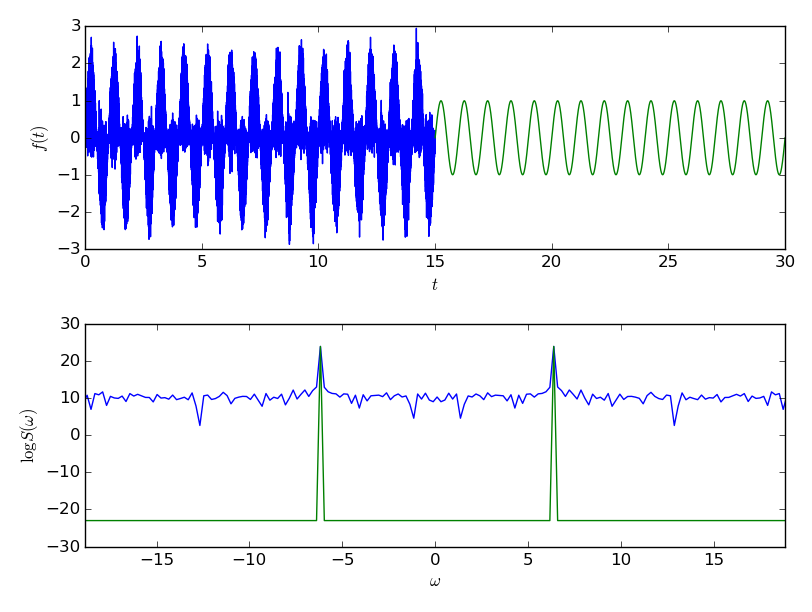
\includegraphics[width=14cm,keepaspectratio=true]{./whitenoise.png}
 \caption{Output of Example \ref{ex:whitenoise}.}
 \label{fig:whitenoise}
\end{figure}

In practice, each noise color requires a different method to be eliminated. Typical cases are the high-pass and low-pass filters, that apply frequency cuts to allow only high and low frequencies, respectively. 

\subsection{Solving ordinary and partial differential equations}
\label{sec:fourierPDE}

There are many different approaches to solve partial differential equations (PDE), which we will discuss in Chapter \ref{chap:PDE}. For now, we shall discuss only the a method using the Fourier transform. As paradigmatic examples, we will use the diffusion equation for the homogeneous case, and the Schrödinger equation for the inhomogeneous case. However, keep in mind that the method used in the Schrödinger equation is also valid for an inhomogeneous diffusion equation.

\subsubsection{Diffusion equation}

Let's consider the homogeneous diffusion equation in one dimension,

\begin{equation}
 \dfrac{\partial}{\partial t}u(x,t) - D \dfrac{\partial^2}{\partial x^2}u(x,t) + v \dfrac{\partial}{\partial x} u(x,t) = 0,
\end{equation}
where $D$ is the diffusion coefficient, $v$ is the drift velocity and $u(x,t)$ is density of the diffusing material (mass, temperature, ...).

In this very simple homogeneous case, the diffusion equation has an analytical solution. For an initial condition $u(x,0) = \delta(x)$,

\begin{equation}
 u(x,t) = \dfrac{1}{2\sqrt{\pi D t}}\exp \left[-\dfrac{(x-vt)^2}{4 D t}\right],
\end{equation}
which is a Gaussian packet with a center that moves as $x = vt$, and broadens with time.

To find this solution, we first take the Fourier transform $x \rightarrow k$ of the diffusion equation,

\begin{equation}
 \dfrac{\partial}{\partial t}\tilde{u}(k,t) + D k^2 \tilde{u}(k,t) + i v k \tilde{u}(k,t) = 0.
\end{equation}
It is easy to show that the solution in $k$-space is $\tilde{u}(k,t) = e^{(-ivk-dk^2)t}\tilde{u}(k,0)$, where $\tilde{u}(k,0)$ is the Fourier transform of the initial condition $u(x,0)$. If the initial condition is $u(x,0) = \delta(x)$, then $\tilde{u}(k,0) = 1/\sqrt{2\pi}$. The inverse Fourier transform can be easily calculated analytically to obtain the solution $u(x,t)$ above.

In this simple case we don't really need any numerical calculation. However, you could eventually face a more general diffusion equation (inhomogeneous, vectorial, coupled, ...) for which numerical methods will be necessary. Therefore, let's illustrate the numerical method assuming that you are able to obtain the solution in $k$-space $\tilde{u}(k,t)$ analytically, but you are not able to calculate the Fourier transform of the initial condition  $\tilde{u}(k,0) =  F[u(x,0)]$ and the inverse Fourier transform to recover $u(x,t) = F^{-1}[\tilde{u}(k,t)]$. The next example solves this problem.

\begin{example}{Diffusion equation}
\label{ex:diffusion}
\begin{minted}[escapeinside=||,mathescape]{julia}
using PyPlot

D = 1; # diffusion coefficient
v = 1; # drift velocity

N = 100; # number of points
L = -10; 
x = linspace(-L, L, N); # x domain
dx = x[2]-x[1]; # x step
k = linspace(-pi/dx, pi/dx, N); # k domain (symmetric)

ux0 = exp(-x.^2); # initial condition $u(x,0)$
uk0 = fftshift(fft(ux0)); # initial condition in k-space $\tilde{u}(k,0)$

# analytical solution in k-space written with the numerical k vector
ukt(t) = exp((-1im*v*k-D*k.^2)*t).*uk0;

# the solution $u(x,t)$ as a function that uses the inverse FFT
uxt(t) = ifft(ifftshift(ukt(t)));

# plot the resuts for different times $t = 0, 1, 2, 3$
clf();
plot(x, ux0);
plot(x, uxt(1));
plot(x, uxt(2));
plot(x, uxt(3));
xlabel(L"$x$");
ylabel(L"$u(x,t)$"];
\end{minted}
\end{example}

\subsubsection{Quantum operators in k-space, the split-step method}

\red{Trying to find an easy way to prove the $\mathcal{O}(\tau^3)$}

Let $H(x,p,t) = T(p,t) + V(x,t)$ be a general Hamiltonian that can be written as a sum of two terms, where the first, $T(p,t)$, is a function of the momentum operator $p = -i\hbar\partial_x$ and the time $t$, while the second, $V(x,t)$, is a function of the position $x$ and time $t$. In general the commutator $[T,V] \neq 0$. We want to solve the time-dependent Schrödinger equation

\begin{equation}
 i\hbar \dfrac{\partial}{\partial t} \psi(x,t) = H(x,p,t)\psi(x,t). 
\end{equation}

For a small time step $\tau$, an approximate numerical solution can be computed as

\begin{equation}
 \psi(x, t+\tau) \approx e^{-i\frac{V\tau}{2\hbar}}  e^{-i\frac{T\tau}{\hbar}}  e^{-i\frac{V\tau}{2\hbar}}\psi(x,t).
\end{equation}
Here we start with half of a time step, $\tau/2$ using V, followed by a full time step $\tau$ using $T$, and another $\tau/2$ to complete the evolution from $t$ to $t+\tau$. This spitting of the operators generates an error of order $\mathcal{O}(\tau^3)$.

More interestingly, this approach can be extremely efficient if we notice that $T$ is a function of momentum $p$, and, therefore, can be better represented in Fourier space (see the derivative property of the Fourier transform). The trick is to carry all operations using $V$ in coordinates space, while those involving $T$ are done in $k$-space. In terms of Fourier transforms, the evolution reads

\begin{equation}
 \psi(x, t+\tau) \approx \exp\left(-i\dfrac{V\tau}{2\hbar}\right) F^{-1}\Big[ \exp\left(-i\dfrac{\tilde{T}\tau}{\hbar}\right)  F\Big[\exp\left(-i\dfrac{V\tau}{2\hbar}\right)  \psi(x,t)\Big]\Big],
\end{equation}
where $\tilde{T} \equiv \tilde{T}(k,t)$ is the Fourier transform $p \rightarrow \hbar k$ of the $T(p,t)$ operator.

Notice that $V(x,t)$ becomes a diagonal matrix when we discretize $x$, but $T(p,t)$ is non-diagonal, as it contains derivatives in the momentum operator. However, in k-space, $\tilde{T}(k,t)$ is diagonal. Therefore, using the Fourier transform as in the equations above, all exponentials will be defined in terms of diagonal matrices, which is easy to calculate. In fact, calculating the exponential of a general matrix is much less efficient than the FFT. Hence the high efficiency of the split-step method. The next example illustrates the difference between the coordinate- and k-space calculations of $\phi = \exp\left(-i\frac{T\tau}{\hbar}\right)\phi_0$, where $T = -\frac{1}{2}p^2$.



\section{Problems}

\begin{problem}{Discrete Fourier Transform}
  \label{prob:DFT}

  Implement your own version of the Discrete Fourier Transform (DFT) in Julia and compare the results with Example \ref{ex:FTShift}. Your implementation will not be efficient and you shall use Julia's native \texttt{fft} function always. However, implementing the DFT will help you learn more about coding.

\end{problem}

\begin{problem}{Derivatives with the FFT package}
  \label{prob:FFTdiff}
  
  Check again Example \ref{ex:FTShift} and adapt it to use the derivative property of the Fourier transforms to calculate the first, second, and third derivatives of a function $f(x)$ set on a discrete domain. Choose a simple function $f(x)$, so that you can find its derivatives analytically and compare with the numeric results.  
 
\end{problem}

\begin{problem}{Pendulum: small vs large amplitudes}
 \label{prob:FFTpendulum}
 
 In the previous chapter, you have written a code to solve the differential equation of a pendulum,
 
 \begin{equation}
   \dfrac{d^2}{dt^2} x(t) = -\omega_0^2 \sin[x(t)] -\gamma v_x(t).
  \end{equation}
 
 For now, let's neglect the damping term, $\gamma = 0$. Consider $\omega_0 = 2\pi$ and the initial conditions $x(0) = x_0$, and $v(0) = 0$. Prepare your code to run over $0 \leq t \leq 100$.
 
 (a) Find $x(t)$ for small amplitudes set by $x_0 = 0.01\pi$ and use the \texttt{fft} command to obtain $\tilde{x}(\omega)$. Plot the spectral function $S(\omega) = |\tilde{x}(\omega)|^2$ for $-2\omega_0 \leq \omega \leq 2\omega_0$.

 (b) Do the same for large amplitudes set by $x_0 = 0.99\pi$.
 
 (c) Discuss the differences between the power spectra of cases (a) and (b).
 
\end{problem}


\begin{problem}{Pendulum: large amplitudes and damping}
 \label{prob:FFTpendulum2}
 
 Consider the same equation an parameters from the previous problem. But now let's start with a large amplitude $x_0 = 0.99\pi$, and a finite damping $\gamma = 0.001$. Solve the differential equation for $0 \leq t \leq 6000$ with a large number of points ($\sim 10^5$). As a function of $t$ you shall see the oscillations loosing amplitude due to the damping.
 
 (a) Plot the spectral function $S(\omega)$ using only the numerical data of $x(t)$ for small $t$, say in a window $0 \leq t \leq 500$.
 
 (b) Plot $S(\omega)$ for the data at large $t$, say in a window $5500 \leq t \leq 6000$.
 
 (c) Explain the difference between the spectral functions.
 
\end{problem}


\begin{problem}{Driven pendulum}
  \label{prob:drivenpendulum}

  Let's analyze the power spectrum of a driven pendulum\cite{pang2006introduction}. Consider a driven pendulum set by 
  
  \begin{equation}
   \dfrac{d^2}{dt^2} x(t) = -\omega_0^2 \sin[x(t)] -\gamma v_x(t) + f_0\cos(\omega_1 t).
  \end{equation}

  (a) Solve this differential equation for $x(0) = 0$, $v_x(0) = 2$, and $0 < t < 3000$, using the parameters $\omega_0 = 1$, $\omega_1 = 2/3$, $\gamma = 1/2$, and $f_0 = 0.9$.
  
  (b) Now try it with the same parameters, except for $f_0 = 1.15$.
  
  (c) The power spectrum is $S(\omega) = |\tilde{x}(\omega)|^2$, where $\tilde{x}(\omega)$ is the Fourier transform ($t \rightarrow \omega$) of $x(t)$. Compare the power spectra of cases (a) and (b). The first is periodic, and will show narrow peaks at the motion frequencies. The second is chaotic, almost all frequencies contribute and the power spectrum is fractal.
  
\end{problem}



